\section{Autonomous Forklift}
\label{sec:agv}
%
The mobile platform is built upon a manual forklift ``CiTi'' from Linde Material Handling. The
forklift is originally equipped with a motorized forks and drive wheel. The forklift has been
retrofitted with a steering mechanism and a commercial AGV control system which is used to interface
the original drive mechanism as well as the steering servo.

To assure safe operation the vehicle is equipped with a standard safety laser scanner (SICK S300)
and an industrial prototype system (RefleX) for detecting workforce using reflective safety
garments. To show the workers the intention of the vehicle, the intend path to be driven with the
required occupied is projected onto the floor. 
%
\subsection{Challenges in Autonomous Navigation}
\label{subsec:AGV_challenges}
%
The industry standard for autonomous navigation of forklifts is to use predefined trajectories where
the trajectories are either manually defined or learned through teaching-by-demonstration from a
human operator~\cite{Hell06,Marsh08}.  Although conceptually simple, fixed trajectories limits the
pallet handling to occur only at predefined fixed poses as well as simple strategies for handling
unforeseen obstacles.  The fundamental difficulties for motion planning of forklifts lies in the the
non-holonomic constraints, the large sweep area it needs to occupy (due to its very non symmetrical
footprint) while operating in limited work space.

To obtain reliable localization in large dynamic warehouses with high accuracy it is commonly used
to mount reflectors in the environment and use a dedicated sensing device~\cite{Hyyp89}. At this
stage natural navigation has successfully been deployed in smaller entities where walls are commonly
observed, however, larger and dynamic environments remains a challenge without additional
infrastructure.
%
\subsection{Navigation}
\label{subsec:navigation}
%
The navigation modules ensures that the forklift is capable of moving save and autonomously through
the work space environment to arbitrary load and unload poses with high accuracy. According to the
AGV system provider Kollmorgen, the required end pose accuracy for picking up pallets is $0.03$~m in
position and $1$~degree (0.017 radians) in orientation. The main component consist of trajectory
generation, tacking controller and a localization system.
 
The trajectory generation on-line is done in two steps, where at first a kinematically feasible path
with discretized start and goal poses are generated using a lattice planner~\cite{Ciri14}. This path
is post-processed using a path smoother~\cite{Andr15} which assure smooth collision-free continuous
trajectory. The tracking of the trajectory is one using a model predictive tracking controller. The
complete navigation system has been implemented, extensively tested and successfully integrated on
the APPLE demonstrator, a detailed description can be found in~\cite{Andr15}.

The localization utilize a Velodyne HDL-32 3D laser
scanner\footnote{\url{http://www.velodynelidar.com/}} which is used to construct a 3D map (using the
3D-NDT-OM map representation) of the static parts of the environment~\cite{Stoy13}. The map and
odometry information is used to localize the vehicle in the presence of dynamic entities using a
dual timescale approach~\cite{Vale14}.

To obtain the pose of the pallet to pickup the current system requires a rough estimate of the
location of the pallet. In order to compute a final estimate based on sensory data from an Asus
Xtion Pro Live\footnote{\url{http://www.asus.com/Multimedia/Xtion_PRO_LIVE/}} mounted on the AGV, a
signed distance function (SDF) tracker~\cite{Cane13} is used with a pre-defined SDF model of the
pallet. The tracking is done while driving towards the provided initial pallet pose and the
trajectory is recomputed on the fly, which depending on the pose offset may include a reverse
operation.
%
\subsection{People Detection}
\label{subsec:people_det}
%
\begin{figure}[t!]
  \begin{center}
    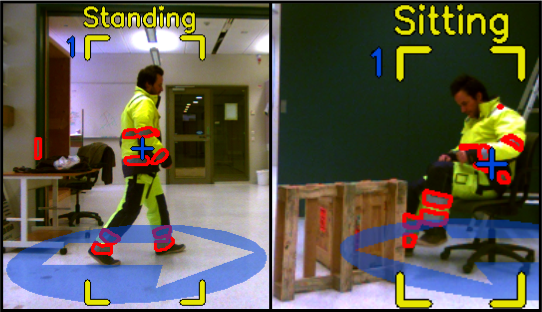
\includegraphics[width =1\linewidth]{figs/person_detection}
    % \vspace{-0.25cm}
    \caption{\textit{People detection:} (Left) the robot picks up an empty pallet in a designated
      zone; (Middle) the robot navigates to a loading zone where a can is detected and picked up;
      (Right) the loaded pallet is transported to a drop-off location.}
    \label{fig:people_det}
    \vspace{-0.5cm}
  \end{center}
\end{figure}
% 
As the envisioned mobile manipulation system will operate in environments shared with human workers,
people detection and human safety are important issues. In APPLE we address the problem by using the
RefleX system we recently developed~\cite{Mosb14}. RefleX is a camera-based on-board safety system
for industrial vehicles and machinery for detection of human workers wearing reflective vests worn
as per safety regulations. The system was designed with industrial safety standards in mind and is
currently being tested as an industrial prototype.
%
